\documentclass[11pt]{article}

% load some asm stuff -
\usepackage{amssymb}
\usepackage{amsmath}
\usepackage{amsthm}
%\usepackage{palatino,lettrine}
\usepackage{fancyhdr}
\usepackage{epsfig}
\usepackage[square,sort,comma,numbers]{natbib}
\usepackage{simplemargins}
\usepackage{setspace}
\usepackage{wrapfig}
\usepackage{hyperref}
%\usepackage{boiboites}
\usepackage[margin=0pt,font=small,labelfont=bf]{caption}
\newcommand{\boldindex}[1]{\textbf{\hyperpage{#1}}}
\usepackage{makeidx}\makeindex

%\bibliographystyle{natbib}
\bibliographystyle{plos2015}

% Set the size
%\textwidth = 6.75 in
%\textheight = 9.75 in
%\oddsidemargin = 0.0 in
%\evensidemargin = 0.0 in
%\topmargin = 0.01 in
%\headheight = 0.0 in
%\headsep = 0.25 in
%\parskip = 0.15in
% \doublespace
\setallmargins{1in}

\newtheorem{example}{Example}[section]
\newtheorem{thm}{Theorem}[section]
\newtheorem{property}{Property}[section]

\theoremstyle{definition}
\newtheorem{defn}[thm]{Definition}

\makeatletter
\renewcommand\subsection{\@startsection
	{subsection}{2}{0mm}
	{-0.05in}
	{-0.5\baselineskip}
	{\normalfont\normalsize\bfseries}}
\renewcommand\subsubsection{\@startsection
	{subsubsection}{2}{0mm}
	{-0.05in}
	{-0.5\baselineskip}
	{\normalfont\normalsize\itshape\bfseries}}
\renewcommand\paragraph{\@startsection
	{paragraph}{2}{0mm}
	{-0.05in}
	{-0.5\baselineskip}
	{\normalfont\normalsize\itshape}}
\makeatother
\linespread{1.1}

\fancypagestyle{proposal}{\fancyhf{}%
	\fancyhead[RO,LE]{\thepage}%
	\fancyhead[LO,RE]{CHEME 131 Module 2 Coupon-Bearing Treasury Securities}%
	\renewcommand\headrulewidth{1pt}}
\pagestyle{proposal}

\usepackage{mdframed}
\definecolor{lgray}{rgb}{0.92,0.92,0.92}
\definecolor{antiquewhite}{rgb}{0.98,0.92,0.84}
\definecolor{lightskyblue}{rgb}{0.93,0.95,0.99}

% defn environment
\mdfdefinestyle{theoremstyle}{% 
    linecolor=black,linewidth=1pt,% 
    frametitlerule=true,% 
    frametitlebackgroundcolor=lgray, 
    innertopmargin=\topskip,} 
\mdtheorem[style=theoremstyle]{definition}{Definition}

% concept environment
\mdfdefinestyle{conceptstyle}{% 
    linecolor=black,linewidth=1pt,% 
    frametitlerule=true,% 
    frametitlebackgroundcolor=antiquewhite, 
    innertopmargin=\topskip,} 
\mdtheorem[style=conceptstyle]{concept}{Concept}
\newcommand{\newterm}[1]{{\it #1}}

% Single space'd bib -
\setlength\bibsep{0pt}

\renewcommand{\rmdefault}{phv}\renewcommand{\sfdefault}{phv}
%\newboxedtheorem[boxcolor=black, background=gray!5,titlebackground=orange!20,titleboxcolor = black]{color_box_example}{Example}{test}

% Change the number format in the ref list -
\renewcommand{\bibnumfmt}[1]{#1.}

% Change Figure to Fig.
\renewcommand{\figurename}{Fig.}
\usepackage{enumitem}
\setlist{noitemsep} % or \setlist{noitemsep} to leave space around whole list

%Joycelyn Chan, Joshua Lequieu, Michael Paull, Chidanand Balaji, Ryan Tasseff
%Our derivation follows closely the earlier development of Fredrickson \citep{Fredrickson:1976fk}.

% Begin ...
\begin{document}

%\begin{titlepage}
{\par\centering\textbf{\Large CHEME 131 Module 2: The Pricing of Coupon Bearing Treasury Securities}}
\vspace{0.2in}
{\par \centering \large{Jeffrey D. Varner}}
\vspace{0.05in}
{\par \centering \large{Smith School of Chemical and Biomolecular Engineering}}
{\par \centering \large{Cornell University, Ithaca NY 14853}}
% \vspace{0.1in}
% {\par \centering \small{Copyright \copyright\ Jeffrey Varner 2018. All Rights Reserved.}}\\

%\end{titlepage}
\date{}
\thispagestyle{empty}

\setcounter{page}{1}

\section*{Introduction}
Previously, we introduced the concept of the time value of money and developed the abstract asset framework to compute the present value of future cash flows.
We used this approach to compute the price of a zero-coupon Treasury bills at auction, 
i.e., the price of a T-bill at the time of purchase that makes the net present value (NPV) equal to zero.
In this module, we expand on the time value of money and develop an approach to compute the price of coupon-bearing Treasury securities.
Unlike T-bills, coupon-bearing Treasury securities pay the holder periodic interest in the form of coupon payments every six months until maturity and the face (par) value of the security at maturity.
Thus, coupon-bearing Treasury securities have multiple cash flow events and can serve as an income stream for the holder.
Further, we explore the relationship between the yield and price of a coupon-bearing Treasury security and conclude with a discussion of potential sources of 
risk associated with these securities.

\section*{Treasury Notes and Bonds}
Previously, we explored United States Treasury Bills or T-bills. Treasury bills are short-term debt instruments with zero coupon payments, 
i.e., there are only two cash flow events with a T-bill: you pay the price of the T-bill at auction, and you receive the face (par) value of the T-bill at maturity. 
In contrast, coupon-bearing Treasury securities are long-term debt instruments that provide a stable interest payment, called a coupon payment, every six months until maturity.
At maturity, the lender also receives the instrument's face (par) value and a final coupon payment.
Let's explore two types of coupon-bearing Treasury securities: Treasury notes and Treasury bonds.
\begin{figure}[h]
    \centering
    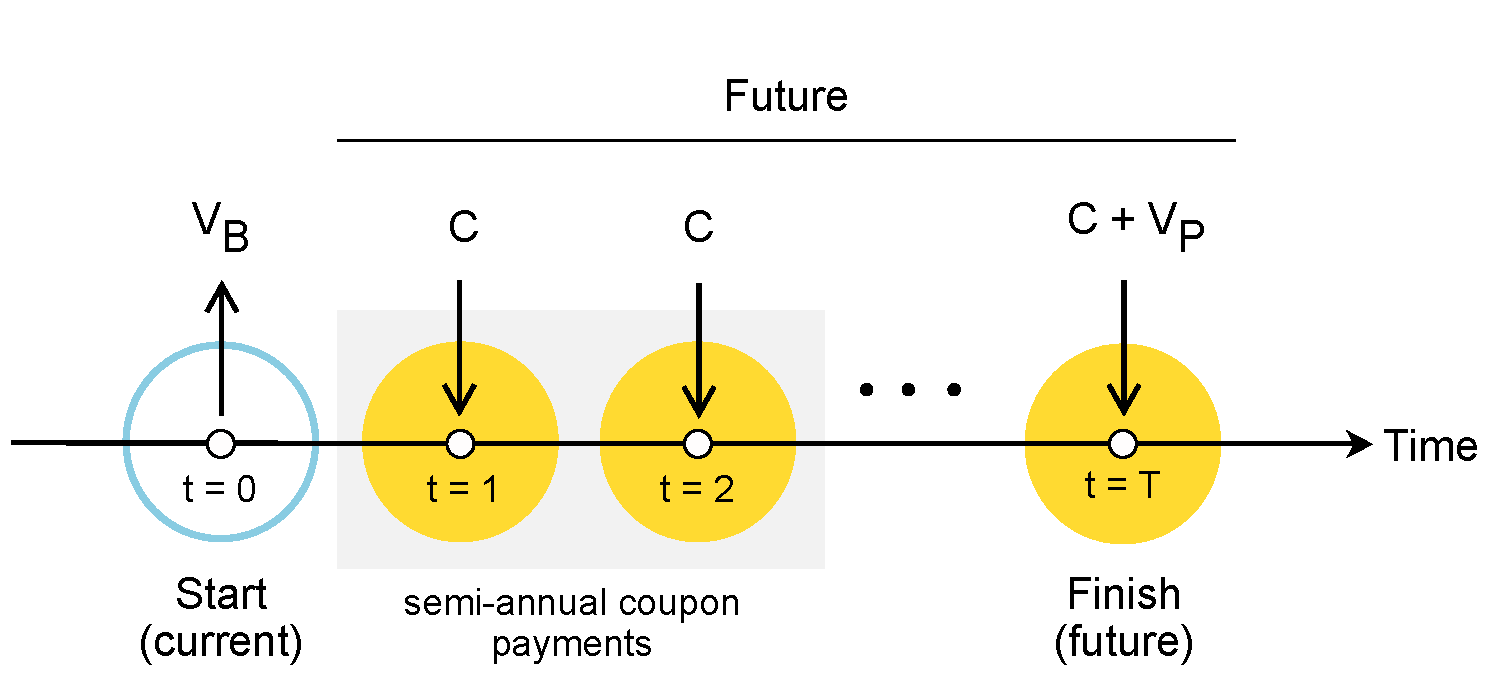
\includegraphics[width=0.85\textwidth]{./figs/Fig-Bond-Asset-Timeline-Schematic.pdf}
    \caption{Asbtract asset schematic of a coupon-bearing Treasury Note (T-note) or Bond (T-bond). 
	The lender (you) gives the United States Treasury 
    the price $V_{B}$ of the note (bond) at auction. In return, the Treasury pays the note (bond) holder (you) the face (par) value of the note (bond) $V_{P}$ at maturity. 
	The schematic is written from the note (bond) holder's perspective (you).}\label{fig:govt-note-bond-schematic}
\end{figure}

\href{https://treasurydirect.gov/marketable-securities/treasury-notes/}{United States Treasury Notes or T-notes}, 
are debt instruments that provide a stable interest payment every six months until maturity, called a coupon payment, and the face (par) value of the note at maturity (Fig. \ref{fig:govt-note-bond-schematic}).
Treasury notes are offered in terms of T = 2, 3, 5, 7, and 10 years and can be bought for more or less than their face (par) value at auction.
 On the other hand,  \href{https://treasurydirect.gov/marketable-securities/treasury-bonds/}{United States Treasury Bonds or T-bonds} 
are coupon debt instruments with more than ten years of maturity, e.g., 20 or 30 years. Similar to notes, bonds are purchased for more or less than their face (par) value and pay interest in the form of coupon payments every six months until maturity.
The coupon rate (interest rate) and the yield (discount factor) for these securities are fixed when they are issued, i.e., at auction, and remain constant over the lifetime of the security.
At maturity, the lender receives the bond's par value (or note) and a final coupon payment. 
Like Treasury bills, the pricing of notes and bonds is based on the present value of the future cash flows. 

\section*{Pricing}
We will use the abstract asset framework to develop a mathematical model for the price of coupon-bearing Treasury securities.
A \texttt{T}-year Treasury note (bond) with face value $V_{P}$, an effective annual discount rate $\bar{r}$, and $\lambda$ coupon payments per year, costs $V_{B}$ at auction.
The note (bond) price is the sum of discounted future coupon payments and face value, making the net present value (NPV) equal to zero:
\begin{equation}
\text{NPV}(T,\bar{r}) = -V_{B} + \mathcal{D}^{-1}_{\lambda{T},0}(\bar{r})\cdot{V_{P}}+C\cdot\sum_{j=1}^{\lambda{T}}\mathcal{D}_{j,0}^{-1}(\bar{r}) = 0
\end{equation}
or equivalently:
\begin{equation}
V_{B} = \mathcal{D}^{-1}_{\lambda{T},0}(\bar{r})\cdot{V_{P}}+C\cdot\sum_{j=1}^{\lambda{T}}\mathcal{D}_{j,0}^{-1}(\bar{r})
\end{equation}
The term $\mathcal{D}_{j,0}^{-1}(\bar{r})$ represents the inverse multistep effective discrete discount factor for period $0\rightarrow{j}$. 
The term $C\equiv(\bar{c}/\lambda)\cdot{V_{P}}$ is the coupon payment, where $\bar{c}$ is the coupon rate (set at auction).
Typically, the coupon rate is quoted as an annual rate, so we divide by $\lambda$ to get the semi-annual coupon payment.
Further, Treasury notes and bonds typically pay coupons every six months, so $\lambda=2$.
Finally, the discounting for Treasury instruments uses a discrete compounding model, so the discount factor for these calculations takes the form:
\begin{equation}
\mathcal{D}_{j,0}(\bar{r}) = \left(1+\frac{\bar{r}}{\lambda}\right)^{j}
\end{equation}
where $j$ denotes the period number, and $\bar{r}$ is the effective yield (constant).

\section*{Sensitivities and Risks}
While United States Treasury securities are considered to be risk-free, they are not without risk. The most obvious risk is the risk of default, i.e., the United States government could default on its obligations and not repay the debt holders (you).
This risk is considered to be very low, and the United States government has never, at least in recent memory, defaulted on its debt obligations (in the absence of technical issues). Other risks are associated with Treasury securities, including inflation and liquidity risks.
However, interest rate risk is the most significant non-default risk associated with Treasury securities.
The price of coupon-bearing Treasury securities is a function of the face (par) value of the security, the coupon rate, the yield (discount rate), and the number of coupon payments per year.
Thus, as these parameters change, e.g., the yield (discount rate), you would expect the price of the Treasury security to change (Concept \ref{concept:malkiel-theorems}):

\begin{concept}[Malkiel's Theorems]\label{concept:malkiel-theorems}
	Malkiel explored the question of bond pricing and proposed five theorems that relate the price of a coupon-bearing Treasury security to changes in these parameters \citep{Malkiel-Bonds-1962}:
\begin{itemize}[leftmargin=*]
\item{\textbf{Theorem 1}: Bond prices move inversely to bond yields.}
\item{\textbf{Theorem 2}: For a given change in yield from the nominal yield, changes in bond prices are greater the longer the term to maturity. }
\item{\textbf{Theorem 3}: The percentage price changes described in Theorem 2 increase at a diminishing rate as N increases. }
\item{\textbf{Theorem 4}: Price movements resulting from equal absolute increases and decreases in yield are asymmetric; i.e., decreasing yields raise bond prices more than the same increase in yields lowers prices. }
\item{\textbf{Theorem 5}: The higher the coupon carried by the bond, the smaller the percentage price fluctuation for a given change in yield, except for one-year securities.}
\end{itemize}
\vspace{0.01in}
\noindent{\textit{Notation}}: when Malkiel refers to the yield, he is referring to the effective annual discount rate, $\bar{r}$. The coupon rate $\bar{c}$ in our bond (note) pricing model is the interest rate.
\end{concept}


The price of a coupon-bearing Treasury security in many ways behaves similar to a T-bill.
Previously, we explored the relationship between the yield (discount rate) and the price of a zero-coupon Treasury bill. 
Theorem 1 tells us that the relationship between the yield and price of a coupon-bearing Treasury security is similar to that of a T-bill, i.e., the cost of the security is inversely related to the yield.
Further, Theorem 2 tells us that the longer the term to maturity, the greater the price change for a given change in yield, which we also saw for T-bills 
in \texttt{Module-1}.
However, the relationship between the yield and price of a coupon-bearing Treasury security may be more complex than that of a T-bill. For example, Theorem 4 tells us that the price of a coupon-bearing Treasury security is more sensitive to a decrease in yield than an increase in yield. Moreover, Theorem 5 suggests the coupon rate (interest rate) may act as a buffer to changes in the price resulting from changes in the yield. We'll explore these ideas in this module's worked example and project.


\section*{Summary}
In this module, we explored the pricing of coupon-bearing Treasury securities.
In particular, we used the abstract asset framework to develop a mathematical model for the price of coupon-bearing United States Treasury notes and bonds.
Notes and bonds are long-term debt instruments that provide a stable interest payment, called a coupon payment, every six months until maturity, and the face (par) value of the note (or bond) at maturity.
These instruments are priced based on the present value of the future cash flows, where the yield (discount factor) and coupon rate for these securities is fixed when they are issued, i.e., at auction and remains constant over the lifetime of the security.

\bibliography{References_v1}

\clearpage
\printindex

\end{document}
